\documentclass[a4paper,14pt]{extarticle}

\usepackage[utf8x]{inputenc}
\usepackage[T1,T2A]{fontenc}
\usepackage[russian]{babel}
\usepackage{hyperref}
\usepackage{indentfirst}
\usepackage{here}
\usepackage{array}
\usepackage[table]{xcolor}
\usepackage{datetime}
\usepackage{multirow}
\usepackage{hhline}
\usepackage{mathtools,cancel}
\usepackage{forest}
\usepackage{graphicx}
\usepackage{caption}
\usepackage{subcaption}
\usepackage{chngcntr}
\usepackage{amsmath}
\usepackage{amssymb}
\usepackage{pgfplots}
\usepackage{pgfplotstable}
\usepackage[left=2cm,right=2cm,top=2cm,bottom=2cm,bindingoffset=0cm]{geometry}
\usepackage{multicol}
\usepackage{askmaps}
\usepackage{tikz}

\newcommand*\circled[1]{\tikz[baseline=(char.base)]{
            \node[shape=circle,draw,inner sep=2pt] (char) {#1};}}

\DeclareMathOperator*{\argmin}{argmin}

\renewcommand{\not}[1]{\mkern 1.5mu\overline{\mkern-1.5mu#1\mkern-1.5mu}\mkern 1.5mu}
\renewcommand{\le}{\ensuremath{\leqslant}}
\renewcommand{\leq}{\ensuremath{\leqslant}}
\renewcommand{\ge}{\ensuremath{\geqslant}}
\renewcommand{\geq}{\ensuremath{\geqslant}}
\renewcommand{\epsilon}{\ensuremath{\varepsilon}}
\renewcommand{\phi}{\ensuremath{\varphi}}

\counterwithin{figure}{section}
\counterwithin{equation}{section}
\counterwithin{table}{section}
\newcommand{\sign}[1][5cm]{\makebox[#1]{\hrulefill}} % Поля подписи и даты
\graphicspath{{pics/}} % Путь до папки с картинками
\captionsetup{justification=centering,margin=1cm}
\def\arraystretch{1.3}

\begin{document}

\begin{titlepage}
\begin{center}
	Санкт-Петербургский политехнический университет Петра Великого\\[0.3cm]
	Институт компьютерных наук и технологий \\[0.3cm]
	Кафедра компьютерных систем и программных технологий\\[4cm]
	
	\textbf{Расчётное задание №6}\\[2mm]
	\textbf{Дисциплина:} Системный анализ и принятие решений\\[2mm]
	\textbf{Тема:} Дискретное программирование. Задача коммивояжёра\\[2mm]
	Вариант 39\\[6.5cm]
\end{center}

\begin{flushleft}
	\hspace*{5mm} Выполнил студент гр. 33501/4  \hspace*{3cm}\sign[3cm]\hspace*{2mm} А.Ю. Ламтев\\
	\hspace*{10.85cm} (подпись)\\[2.5mm]
	\hspace*{5mm} Преподаватель \hspace*{6.45cm}\sign[3cm]\hspace*{2mm} С.С. Сабонис\\
	\hspace*{10.85cm} (подпись)\\[2.5mm]
	\hspace*{11.1cm} <<\underline{\the\day}>> \underline{\hspace{5mm}ноября\hspace{5mm}} \the\year\hspace{1mm} г.
\end{flushleft}

\vfill

\begin{center}
	Санкт-Петербург\\
	\the\year
\end{center}
\end{titlepage}
\addtocounter{page}{1}

\section{Задание}

Дана задача нелинейного программирования:

\begin{displaymath}
	max \left( -17 x^2_1 - 23 x^2_2 + 8 x_1 x_2 + 182 x_1 + 266 x_2 \right)
\end{displaymath}

\begin{enumerate}

	\item Записать условие оптимальности и решить задачу аналитически.
	
	\item Решить задачу методом релаксации.
	
	\item Решить задачу методом наискорейшего подъема.
	
	\item Решить задачу методом Ньютона.	
	
	\item Решить задачу методом сопряжённых градиентов.

	\item Решить задачу методом Бройдена.

\end{enumerate}

Решить задачу методами 2 -- 6, выбрав ещё 3 начальных точки. Графики сгруппировать по методам: на одном графике траектории поиска решения задачи из четырёх разных начальных точек одним методом, на другом графике – другим методом и т.д. 

\section{Решение}

\subsection{Аналитическое решение}

Решим задачу аналитически. Для этого запишем условие оптимальности:

\begin{equation}
\label{eq:opt-cond}
	\nabla f(X) \Big|_{X = X^*} = \left(  \frac{\partial f}{\partial x_1}(X) \hspace{7mm} \frac{\partial f}{\partial x_2}(X) \right)^T \Big|_{X = X^*} = 0, \hspace{5mm} X = 
	%
	\begin{pmatrix}
		x_1
		\\
		x_2
	\end{pmatrix}
\end{equation}

Вычислим частные производные первого порядка целевой функции:

\begin{equation*}
	\frac{\partial f}{\partial x_1}(X) = -34 x_1 + 8 x_2 + 182
\end{equation*}

\begin{equation*}
	\frac{\partial f}{\partial x_2}(X) = -46 x_2 + 8 x_1 + 266
\end{equation*}

Подставим их в уравнение \ref{eq:opt-cond} и решим полученную систему уравнений:

\begin{equation*}
	\begin{pmatrix}
		-34 x_1 + 8 x_2 + 182
		\\
		-46 x_2 + 8 x_1 + 266
	\end{pmatrix}
	%
	= 0
	%
	\Rightarrow
	\begin{pmatrix}
		-34 & 8
		\\
		-46 & 8 x_1
	\end{pmatrix}
	\cdot X^* =
	\begin{pmatrix}
		-182
		\\
		-266
	\end{pmatrix}
	\Rightarrow
\end{equation*}

\begin{equation*}
	\Rightarrow X^* = 
	\begin{pmatrix}
		7
		\\
		7
	\end{pmatrix}
	\text{ -- оптимальная точка}
\end{equation*}

Запишем достаточное условие максимума:

\begin{equation}
\label{eq:enough-cond}
	H(X) \Big|_{X=X^*} = 
	\begin{pmatrix}
		\frac{\partial^2 f}{\partial x^2_1}(X) && \frac{\partial^2 f}{\partial x_1 \partial x_2}(X)
		\\
		\frac{\partial^2 f}{\partial x_1 \partial x_2}(X) && \frac{\partial^2 f}{\partial x^2_2}(X)
	\end{pmatrix}
	\Big|_{X=X^*}
	\text{-- отрицательно определена}
\end{equation}

Вычислим частные производные второго порядка целевой функции:

\begin{equation*}
	\frac{\partial^2 f}{\partial x^2_1}(X) = -34
\end{equation*}

\begin{equation*}
	\frac{\partial^2 f}{\partial x_1 \partial x_2}(X) = 8
\end{equation*}

\begin{equation*}
	\frac{\partial^2 f}{\partial x^2_2}(X) = - 46
\end{equation*}

Подставим их в уравнение \ref{eq:enough-cond} и получим:

\begin{equation*}
	H(X) = const(X) =
	\begin{pmatrix}
		-34 && 8
		\\
		8 && -46
	\end{pmatrix}
\end{equation*}

Согласно критерию Сильвестра (действительная квадратичная форма является отрицательно определенной тогда и только тогда, когда знаки главных миноров ее матрицы чередуются, причем $\Delta_1 < 0$), полученная матрица Гессе отрицательно определена, т.к $\Delta_1 = h_{11} = -34 < 0$ и $\Delta_2 =%
\begin{vmatrix}% 
	h_{11} & h_{12}%
	\\
	h_{21} & h_{22}
\end{vmatrix} = \\
=
\begin{vmatrix}% 
	-34 & 8%
	\\
	8 & -46
\end{vmatrix} =1500 > 0$

Следовательно $X^* = \begin{pmatrix}
	7
	\\
	7
\end{pmatrix}$ -- решение.

\subsection{Метод релаксации}

Решим задачу методом релаксации для четырёх разных начальных точек: $X_1^{(0)} = (0, 0)$, $X_2^{(0)} = (3, 5)$, $X_3^{(0)} = (9, 10)$, $X_4^{(0)} = (14, 6)$.\\

Для этого разработаем прорграмму на языке программирования \textbf{Python} c использованием стандартной библиотеки и пакетов \textbf{NumPy}, \textbf{CSV}, \textbf{Matplotlib}, которая реализует данный метод и позволит визуализировать результаты в виде таблиц и графиков.  Исходный код приведён в \hyperref[sec:application]{приложении}.\\

В таблицах \ref{tab:trajectory-relax-0} -- \ref{tab:trajectory-relax-3} приведены траектории поиска решения для всех начальных точек.

\begin{table}[H]
\begin{center}
	\caption{Траектория поиска решения при $X_1^{(0)} = (0, 0)$}
	\label{tab:trajectory-relax-0}
	\def\tabcolsep{10pt}
	\def\arraystretch{1.23}
	\fontsize{13}{14}\selectfont
	\pgfplotstabletypeset[col sep=comma,
	    columns={it, x1, x2, f},
	    column type/.add={|c|c|c|c|}{},
	    columns/it/.style={fixed, precision=0, zerofill, column name={Итерация}},
	    columns/x1/.style={fixed, precision=5, zerofill, column name={$x_1$}},
	    columns/x2/.style={fixed, precision=5, zerofill, column name={$x_2$}},
	    columns/f/.style={fixed, precision=5, zerofill, column name={$f(x_1, x_2)$}},
	    every nth row={1}{before row=\hline},
	    every head row/.style={before row=\hline, after row=\hline},
	    every last row/.style={after row=\hline}
	   ]{data/relax0.csv}
\end{center}
\end{table}

\begin{table}[H]
\begin{center}
	\caption{Траектория поиска решения при $X_2^{(0)} = (3, 5)$}
	\label{tab:trajectory-relax-1}
	\def\tabcolsep{10pt}
	\def\arraystretch{1.23}
	\fontsize{13}{14}\selectfont
	\pgfplotstabletypeset[col sep=comma,
	    columns={it, x1, x2, f},
	    column type/.add={|c|c|c|c|}{},
	    columns/it/.style={fixed, precision=0, zerofill, column name={Итерация}},
	    columns/x1/.style={fixed, precision=5, zerofill, column name={$x_1$}},
	    columns/x2/.style={fixed, precision=5, zerofill, column name={$x_2$}},
	    columns/f/.style={fixed, precision=5, zerofill, column name={$f(x_1, x_2)$}},
	    every nth row={1}{before row=\hline},
	    every head row/.style={before row=\hline, after row=\hline},
	    every last row/.style={after row=\hline}
	   ]{data/relax1.csv}
\end{center}
\end{table}

\begin{table}[H]
\begin{center}
	\caption{Траектория поиска решения при $X_3^{(0)} = (9, 10)$}
	\label{tab:trajectory-relax-2}
	\def\tabcolsep{10pt}
	\def\arraystretch{1.23}
	\fontsize{13}{14}\selectfont
	\pgfplotstabletypeset[col sep=comma,
	    columns={it, x1, x2, f},
	    column type/.add={|c|c|c|c|}{},
	    columns/it/.style={fixed, precision=0, zerofill, column name={Итерация}},
	    columns/x1/.style={fixed, precision=5, zerofill, column name={$x_1$}},
	    columns/x2/.style={fixed, precision=5, zerofill, column name={$x_2$}},
	    columns/f/.style={fixed, precision=5, zerofill, column name={$f(x_1, x_2)$}},
	    every nth row={1}{before row=\hline},
	    every head row/.style={before row=\hline, after row=\hline},
	    every last row/.style={after row=\hline}
	   ]{data/relax2.csv}
\end{center}
\end{table}

\begin{table}[H]
\begin{center}
	\caption{Траектория поиска решения при $X_3^{(0)} = (14, 6)$}
	\label{tab:trajectory-relax-3}
	\def\tabcolsep{10pt}
	\def\arraystretch{1.23}
	\fontsize{13}{14}\selectfont
	\pgfplotstabletypeset[col sep=comma,
	    columns={it, x1, x2, f},
	    column type/.add={|c|c|c|c|}{},
	    columns/it/.style={fixed, precision=0, zerofill, column name={Итерация}},
	    columns/x1/.style={fixed, precision=5, zerofill, column name={$x_1$}},
	    columns/x2/.style={fixed, precision=5, zerofill, column name={$x_2$}},
	    columns/f/.style={fixed, precision=5, zerofill, column name={$f(x_1, x_2)$}},
	    every nth row={1}{before row=\hline},
	    every head row/.style={before row=\hline, after row=\hline},
	    every last row/.style={after row=\hline}
	   ]{data/relax3.csv}
\end{center}
\end{table}

Решение задачи для всех выбранных начальных точек сошлось к\\ $X^* = (7, 7)$ и $f(X^*) = 1568$.\\

На рис. \ref{pic:relax} представлен график решения задачи.

\begin{figure}[H]
\begin{center}
	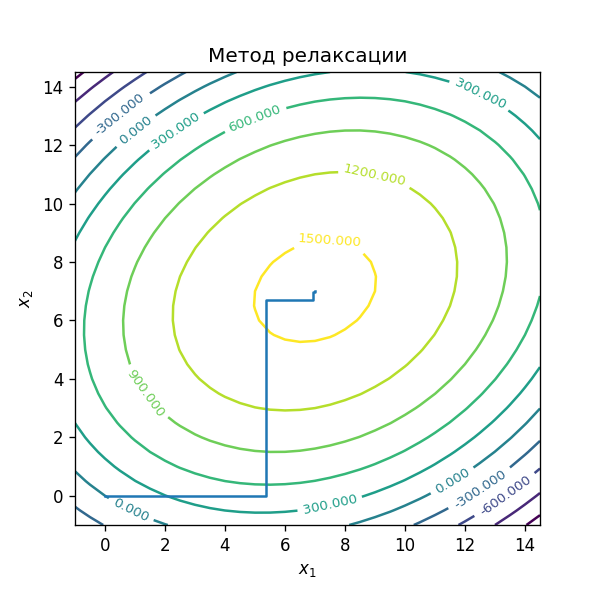
\includegraphics[scale=1]{relax}
	\caption{Линии равного уровня целевой функции и траектории поиска решения}
	\label{pic:relax}
\end{center}
\end{figure}


\subsection{Метод наискорейшего подъёма}

Решим задачу методом наискорейшего подъёма для четырёх разных начальных точек: $X_1^{(0)} = (0, 0)$, $X_2^{(0)} = (3, 5)$, $X_3^{(0)} = (9, 10)$, $X_4^{(0)} = (14, 6)$.\\

Для этого разработаем прорграмму на языке программирования \textbf{Python} c использованием стандартной библиотеки и пакетов \textbf{NumPy}, \textbf{CSV}, \textbf{Matplotlib}, которая реализует данный метод и позволит визуализировать результаты в виде таблиц и графиков.  Исходный код приведён в \hyperref[sec:application]{приложении}.\\

В таблицах \ref{tab:trajectory-gd-0} -- \ref{tab:trajectory-gd-3} приведены траектории поиска решения для всех начальных точек.

\begin{table}[H]
\begin{center}
	\caption{Траектория поиска решения при $X_1^{(0)} = (0, 0)$}
	\label{tab:trajectory-gd-0}
	\def\tabcolsep{10pt}
	\def\arraystretch{1.23}
	\fontsize{13}{14}\selectfont
	\pgfplotstabletypeset[col sep=comma,
	    columns={it, x1, x2, f},
	    column type/.add={|c|c|c|c|}{},
	    columns/it/.style={fixed, precision=0, zerofill, column name={Итерация}},
	    columns/x1/.style={fixed, precision=5, zerofill, column name={$x_1$}},
	    columns/x2/.style={fixed, precision=5, zerofill, column name={$x_2$}},
	    columns/f/.style={fixed, precision=5, zerofill, column name={$f(x_1, x_2)$}},
	    every nth row={1}{before row=\hline},
	    every head row/.style={before row=\hline, after row=\hline},
	    every last row/.style={after row=\hline}
	   ]{data/gd0.csv}
\end{center}
\end{table}

\begin{table}[H]
\begin{center}
	\caption{Траектория поиска решения при $X_2^{(0)} = (3, 5)$}
	\label{tab:trajectory-gd-1}
	\def\tabcolsep{10pt}
	\def\arraystretch{1.23}
	\fontsize{13}{14}\selectfont
	\pgfplotstabletypeset[col sep=comma,
	    columns={it, x1, x2, f},
	    column type/.add={|c|c|c|c|}{},
	    columns/it/.style={fixed, precision=0, zerofill, column name={Итерация}},
	    columns/x1/.style={fixed, precision=5, zerofill, column name={$x_1$}},
	    columns/x2/.style={fixed, precision=5, zerofill, column name={$x_2$}},
	    columns/f/.style={fixed, precision=5, zerofill, column name={$f(x_1, x_2)$}},
	    every nth row={1}{before row=\hline},
	    every head row/.style={before row=\hline, after row=\hline},
	    every last row/.style={after row=\hline}
	   ]{data/gd1.csv}
\end{center}
\end{table}

\begin{table}[H]
\begin{center}
	\caption{Траектория поиска решения при $X_3^{(0)} = (9, 10)$}
	\label{tab:trajectory-gd-2}
	\def\tabcolsep{10pt}
	\def\arraystretch{1.23}
	\fontsize{13}{14}\selectfont
	\pgfplotstabletypeset[col sep=comma,
	    columns={it, x1, x2, f},
	    column type/.add={|c|c|c|c|}{},
	    columns/it/.style={fixed, precision=0, zerofill, column name={Итерация}},
	    columns/x1/.style={fixed, precision=5, zerofill, column name={$x_1$}},
	    columns/x2/.style={fixed, precision=5, zerofill, column name={$x_2$}},
	    columns/f/.style={fixed, precision=5, zerofill, column name={$f(x_1, x_2)$}},
	    every nth row={1}{before row=\hline},
	    every head row/.style={before row=\hline, after row=\hline},
	    every last row/.style={after row=\hline}
	   ]{data/gd2.csv}
\end{center}
\end{table}

\begin{table}[H]
\begin{center}
	\caption{Траектория поиска решения при $X_3^{(0)} = (14, 6)$}
	\label{tab:trajectory-gd-3}
	\def\tabcolsep{10pt}
	\def\arraystretch{1.23}
	\fontsize{13}{14}\selectfont
	\pgfplotstabletypeset[col sep=comma,
	    columns={it, x1, x2, f},
	    column type/.add={|c|c|c|c|}{},
	    columns/it/.style={fixed, precision=0, zerofill, column name={Итерация}},
	    columns/x1/.style={fixed, precision=5, zerofill, column name={$x_1$}},
	    columns/x2/.style={fixed, precision=5, zerofill, column name={$x_2$}},
	    columns/f/.style={fixed, precision=5, zerofill, column name={$f(x_1, x_2)$}},
	    every nth row={1}{before row=\hline},
	    every head row/.style={before row=\hline, after row=\hline},
	    every last row/.style={after row=\hline}
	   ]{data/gd3.csv}
\end{center}
\end{table}

Решение задачи для всех выбранных начальных точек сошлось к\\ $X^* = (7, 7)$ и $f(X^*) = 1568$.\\

На рис. \ref{pic:gd} представлен график решения задачи.

\begin{figure}[H]
\begin{center}
	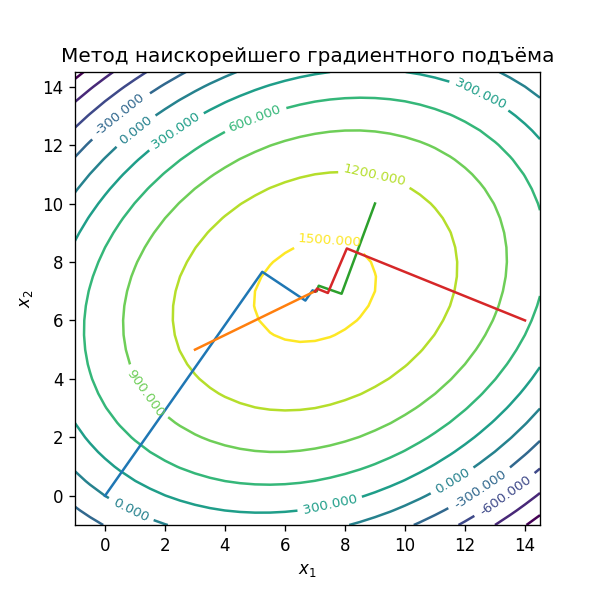
\includegraphics[scale=0.89]{gd}
	\caption{Линии равного уровня целевой функции и траектории поиска решения}
	\label{pic:gd}
\end{center}
\end{figure}

\subsection{Метод Ньютона}

Решим задачу методом Ньютона для четырёх разных начальных точек: $X_1^{(0)} = (0, 0)$, $X_2^{(0)} = (3, 5)$, $X_3^{(0)} = (9, 10)$, $X_4^{(0)} = (14, 6)$.\\

Для этого разработаем прорграмму на языке программирования \textbf{Python} c использованием стандартной библиотеки и пакетов \textbf{NumPy}, \textbf{CSV}, \textbf{Matplotlib}, которая реализует данный метод и позволит визуализировать результаты в виде таблиц и графиков.  Исходный код приведён в \hyperref[sec:application]{приложении}.\\

В таблицах \ref{tab:trajectory-newton-0} -- \ref{tab:trajectory-newton-3} приведены траектории поиска решения для всех начальных точек.

\begin{table}[H]
\begin{center}
	\caption{Траектория поиска решения при $X_1^{(0)} = (0, 0)$}
	\label{tab:trajectory-newton-0}
	\def\tabcolsep{10pt}
	\def\arraystretch{1.23}
	\fontsize{13}{14}\selectfont
	\pgfplotstabletypeset[col sep=comma,
	    columns={it, x1, x2, f},
	    column type/.add={|c|c|c|c|}{},
	    columns/it/.style={fixed, precision=0, zerofill, column name={Итерация}},
	    columns/x1/.style={fixed, precision=4, zerofill, column name={$x_1$}},
	    columns/x2/.style={fixed, precision=4, zerofill, column name={$x_2$}},
	    columns/f/.style={fixed, precision=4, zerofill, column name={$f(x_1, x_2)$}},
	    every nth row={1}{before row=\hline},
	    every head row/.style={before row=\hline, after row=\hline},
	    every last row/.style={after row=\hline}
	   ]{data/newton0.csv}
\end{center}
\end{table}

\begin{table}[H]
\begin{center}
	\caption{Траектория поиска решения при $X_2^{(0)} = (3, 5)$}
	\label{tab:trajectory-newton-1}
	\def\tabcolsep{10pt}
	\def\arraystretch{1.23}
	\fontsize{13}{14}\selectfont
	\pgfplotstabletypeset[col sep=comma,
	    columns={it, x1, x2, f},
	    column type/.add={|c|c|c|c|}{},
	    columns/it/.style={fixed, precision=0, zerofill, column name={Итерация}},
	    columns/x1/.style={fixed, precision=4, zerofill, column name={$x_1$}},
	    columns/x2/.style={fixed, precision=4, zerofill, column name={$x_2$}},
	    columns/f/.style={fixed, precision=4, zerofill, column name={$f(x_1, x_2)$}},
	    every nth row={1}{before row=\hline},
	    every head row/.style={before row=\hline, after row=\hline},
	    every last row/.style={after row=\hline}
	   ]{data/newton1.csv}
\end{center}
\end{table}

\begin{table}[H]
\begin{center}
	\caption{Траектория поиска решения при $X_3^{(0)} = (9, 10)$}
	\label{tab:trajectory-newton-2}
	\def\tabcolsep{10pt}
	\def\arraystretch{1.23}
	\fontsize{13}{14}\selectfont
	\pgfplotstabletypeset[col sep=comma,
	    columns={it, x1, x2, f},
	    column type/.add={|c|c|c|c|}{},
	    columns/it/.style={fixed, precision=0, zerofill, column name={Итерация}},
	    columns/x1/.style={fixed, precision=4, zerofill, column name={$x_1$}},
	    columns/x2/.style={fixed, precision=4, zerofill, column name={$x_2$}},
	    columns/f/.style={fixed, precision=4, zerofill, column name={$f(x_1, x_2)$}},
	    every nth row={1}{before row=\hline},
	    every head row/.style={before row=\hline, after row=\hline},
	    every last row/.style={after row=\hline}
	   ]{data/newton2.csv}
\end{center}
\end{table}

\begin{table}[H]
\begin{center}
	\caption{Траектория поиска решения при $X_3^{(0)} = (14, 6)$}
	\label{tab:trajectory-newton-3}
	\def\tabcolsep{10pt}
	\def\arraystretch{1.23}
	\fontsize{13}{14}\selectfont
	\pgfplotstabletypeset[col sep=comma,
	    columns={it, x1, x2, f},
	    column type/.add={|c|c|c|c|}{},
	    columns/it/.style={fixed, precision=0, zerofill, column name={Итерация}},
	    columns/x1/.style={fixed, precision=4, zerofill, column name={$x_1$}},
	    columns/x2/.style={fixed, precision=4, zerofill, column name={$x_2$}},
	    columns/f/.style={fixed, precision=4, zerofill, column name={$f(x_1, x_2)$}},
	    every nth row={1}{before row=\hline},
	    every head row/.style={before row=\hline, after row=\hline},
	    every last row/.style={after row=\hline}
	   ]{data/newton3.csv}
\end{center}
\end{table}

Решение задачи для всех выбранных начальных точек сошлось к\\ $X^* = (7, 7)$ и $f(X^*) = 1568$.\\

На рис. \ref{pic:newton} представлен график решения задачи.

\begin{figure}[H]
\begin{center}
	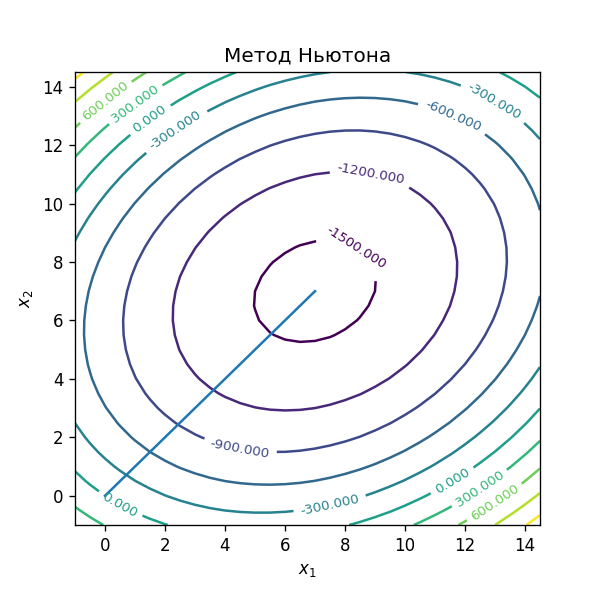
\includegraphics[scale=1]{newton}
	\caption{Линии равного уровня целевой функции и траектории поиска решения}
	\label{pic:newton}
\end{center}
\end{figure}

\subsection{Метод сопряжённых градиентов}

Решим задачу методом сопряжённых градиентов для четырёх разных начальных точек: $X_1^{(0)} = (0, 0)$, $X_2^{(0)} = (3, 5)$, $X_3^{(0)} = (9, 10)$, $X_4^{(0)} = (14, 6)$.\\

Для этого разработаем прорграмму на языке программирования \textbf{Python} c использованием стандартной библиотеки и пакетов \textbf{NumPy}, \textbf{CSV}, \textbf{Matplotlib}, которая реализует данный метод и позволит визуализировать результаты в виде таблиц и графиков.  Исходный код приведён в \hyperref[sec:application]{приложении}.\\

В таблицах \ref{tab:trajectory-cg-0} -- \ref{tab:trajectory-cg-3} приведены траектории поиска решения для всех начальных точек.

\begin{table}[H]
\begin{center}
	\caption{Траектория поиска решения при $X_1^{(0)} = (0, 0)$}
	\label{tab:trajectory-cg-0}
	\def\tabcolsep{10pt}
	\def\arraystretch{1.23}
	\fontsize{13}{14}\selectfont
	\pgfplotstabletypeset[col sep=comma,
	    columns={it, x1, x2, f},
	    column type/.add={|c|c|c|c|}{},
	    columns/it/.style={fixed, precision=0, zerofill, column name={Итерация}},
	    columns/x1/.style={fixed, precision=4, zerofill, column name={$x_1$}},
	    columns/x2/.style={fixed, precision=4, zerofill, column name={$x_2$}},
	    columns/f/.style={fixed, precision=4, zerofill, column name={$f(x_1, x_2)$}},
	    every nth row={1}{before row=\hline},
	    every head row/.style={before row=\hline, after row=\hline},
	    every last row/.style={after row=\hline}
	   ]{data/cg0.csv}
\end{center}
\end{table}

\begin{table}[H]
\begin{center}
	\caption{Траектория поиска решения при $X_2^{(0)} = (3, 5)$}
	\label{tab:trajectory-cg-1}
	\def\tabcolsep{10pt}
	\def\arraystretch{1.23}
	\fontsize{13}{14}\selectfont
	\pgfplotstabletypeset[col sep=comma,
	    columns={it, x1, x2, f},
	    column type/.add={|c|c|c|c|}{},
	    columns/it/.style={fixed, precision=0, zerofill, column name={Итерация}},
	    columns/x1/.style={fixed, precision=4, zerofill, column name={$x_1$}},
	    columns/x2/.style={fixed, precision=4, zerofill, column name={$x_2$}},
	    columns/f/.style={fixed, precision=4, zerofill, column name={$f(x_1, x_2)$}},
	    every nth row={1}{before row=\hline},
	    every head row/.style={before row=\hline, after row=\hline},
	    every last row/.style={after row=\hline}
	   ]{data/cg1.csv}
\end{center}
\end{table}

\begin{table}[H]
\begin{center}
	\caption{Траектория поиска решения при $X_3^{(0)} = (9, 10)$}
	\label{tab:trajectory-cg-2}
	\def\tabcolsep{10pt}
	\def\arraystretch{1.23}
	\fontsize{13}{14}\selectfont
	\pgfplotstabletypeset[col sep=comma,
	    columns={it, x1, x2, f},
	    column type/.add={|c|c|c|c|}{},
	    columns/it/.style={fixed, precision=0, zerofill, column name={Итерация}},
	    columns/x1/.style={fixed, precision=4, zerofill, column name={$x_1$}},
	    columns/x2/.style={fixed, precision=4, zerofill, column name={$x_2$}},
	    columns/f/.style={fixed, precision=4, zerofill, column name={$f(x_1, x_2)$}},
	    every nth row={1}{before row=\hline},
	    every head row/.style={before row=\hline, after row=\hline},
	    every last row/.style={after row=\hline}
	   ]{data/cg2.csv}
\end{center}
\end{table}

\begin{table}[H]
\begin{center}
	\caption{Траектория поиска решения при $X_3^{(0)} = (14, 6)$}
	\label{tab:trajectory-cg-3}
	\def\tabcolsep{10pt}
	\def\arraystretch{1.23}
	\fontsize{13}{14}\selectfont
	\pgfplotstabletypeset[col sep=comma,
	    columns={it, x1, x2, f},
	    column type/.add={|c|c|c|c|}{},
	    columns/it/.style={fixed, precision=0, zerofill, column name={Итерация}},
	    columns/x1/.style={fixed, precision=4, zerofill, column name={$x_1$}},
	    columns/x2/.style={fixed, precision=4, zerofill, column name={$x_2$}},
	    columns/f/.style={fixed, precision=4, zerofill, column name={$f(x_1, x_2)$}},
	    every nth row={1}{before row=\hline},
	    every head row/.style={before row=\hline, after row=\hline},
	    every last row/.style={after row=\hline}
	   ]{data/cg3.csv}
\end{center}
\end{table}

Решение задачи для всех выбранных начальных точек сошлось к\\ $X^* = (7, 7)$ и $f(X^*) = 1568$.\\

На рис. \ref{pic:cg} представлен график решения задачи.

\begin{figure}[H]
\begin{center}
	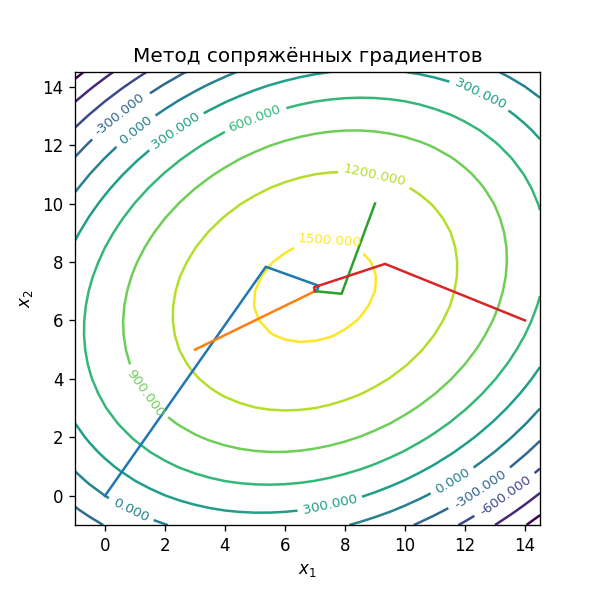
\includegraphics[scale=1]{cg}
	\caption{Линии равного уровня целевой функции и траектории поиска решения}
	\label{pic:cg}
\end{center}
\end{figure}

\subsection{Метод Бройдена}

Решим задачу методом Бройдена для четырёх разных начальных точек: $X_1^{(0)} = (0, 0)$, $X_2^{(0)} = (3, 5)$, $X_3^{(0)} = (9, 10)$, $X_4^{(0)} = (14, 6)$.\\

Для этого разработаем прорграмму на языке программирования \textbf{Python} c использованием стандартной библиотеки и пакетов \textbf{NumPy}, \textbf{CSV}, \textbf{Matplotlib}, которая реализует данный метод и позволит визуализировать результаты в виде таблиц и графиков.  Исходный код приведён в \hyperref[sec:application]{приложении}.\\

В таблицах \ref{tab:trajectory-broyden-0} -- \ref{tab:trajectory-broyden-3} приведены траектории поиска решения для всех начальных точек.

\begin{table}[H]
\begin{center}
	\caption{Траектория поиска решения при $X_1^{(0)} = (0, 0)$}
	\label{tab:trajectory-broyden-0}
	\def\tabcolsep{10pt}
	\def\arraystretch{1.23}
	\fontsize{13}{14}\selectfont
	\pgfplotstabletypeset[col sep=comma,
	    columns={it, x1, x2, f},
	    column type/.add={|c|c|c|c|}{},
	    columns/it/.style={fixed, precision=0, zerofill, column name={Итерация}},
	    columns/x1/.style={fixed, precision=5, zerofill, column name={$x_1$}},
	    columns/x2/.style={fixed, precision=5, zerofill, column name={$x_2$}},
	    columns/f/.style={fixed, precision=5, zerofill, column name={$f(x_1, x_2)$}},
	    every nth row={1}{before row=\hline},
	    every head row/.style={before row=\hline, after row=\hline},
	    every last row/.style={after row=\hline}
	   ]{data/broyden0.csv}
\end{center}
\end{table}

\begin{table}[H]
\begin{center}
	\caption{Траектория поиска решения при $X_2^{(0)} = (3, 5)$}
	\label{tab:trajectory-broyden-1}
	\def\tabcolsep{10pt}
	\def\arraystretch{1.23}
	\fontsize{13}{14}\selectfont
	\pgfplotstabletypeset[col sep=comma,
	    columns={it, x1, x2, f},
	    column type/.add={|c|c|c|c|}{},
	    columns/it/.style={fixed, precision=0, zerofill, column name={Итерация}},
	    columns/x1/.style={fixed, precision=5, zerofill, column name={$x_1$}},
	    columns/x2/.style={fixed, precision=5, zerofill, column name={$x_2$}},
	    columns/f/.style={fixed, precision=5, zerofill, column name={$f(x_1, x_2)$}},
	    every nth row={1}{before row=\hline},
	    every head row/.style={before row=\hline, after row=\hline},
	    every last row/.style={after row=\hline}
	   ]{data/broyden1.csv}
\end{center}
\end{table}

\begin{table}[H]
\begin{center}
	\caption{Траектория поиска решения при $X_3^{(0)} = (9, 10)$}
	\label{tab:trajectory-broyden-2}
	\def\tabcolsep{10pt}
	\def\arraystretch{1.23}
	\fontsize{13}{14}\selectfont
	\pgfplotstabletypeset[col sep=comma,
	    columns={it, x1, x2, f},
	    column type/.add={|c|c|c|c|}{},
	    columns/it/.style={fixed, precision=0, zerofill, column name={Итерация}},
	    columns/x1/.style={fixed, precision=5, zerofill, column name={$x_1$}},
	    columns/x2/.style={fixed, precision=5, zerofill, column name={$x_2$}},
	    columns/f/.style={fixed, precision=5, zerofill, column name={$f(x_1, x_2)$}},
	    every nth row={1}{before row=\hline},
	    every head row/.style={before row=\hline, after row=\hline},
	    every last row/.style={after row=\hline}
	   ]{data/broyden2.csv}
\end{center}
\end{table}

\begin{table}[H]
\begin{center}
	\caption{Траектория поиска решения при $X_3^{(0)} = (14, 6)$}
	\label{tab:trajectory-broyden-3}
	\def\tabcolsep{10pt}
	\def\arraystretch{1.23}
	\fontsize{13}{14}\selectfont
	\pgfplotstabletypeset[col sep=comma,
	    columns={it, x1, x2, f},
	    column type/.add={|c|c|c|c|}{},
	    columns/it/.style={fixed, precision=0, zerofill, column name={Итерация}},
	    columns/x1/.style={fixed, precision=5, zerofill, column name={$x_1$}},
	    columns/x2/.style={fixed, precision=5, zerofill, column name={$x_2$}},
	    columns/f/.style={fixed, precision=5, zerofill, column name={$f(x_1, x_2)$}},
	    every nth row={1}{before row=\hline},
	    every head row/.style={before row=\hline, after row=\hline},
	    every last row/.style={after row=\hline}
	   ]{data/broyden3.csv}
\end{center}
\end{table}

Решение задачи для всех выбранных начальных точек сошлось к\\ $X^* = (7, 7)$ и $f(X^*) = 1568$.\\

На рис. \ref{pic:broyden} представлен график решения задачи.

\begin{figure}[H]
\begin{center}
	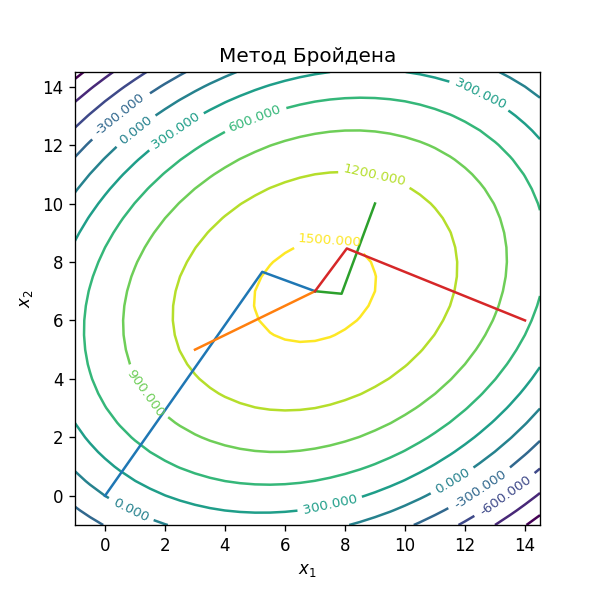
\includegraphics[scale=1]{broyden}
	\caption{Линии равного уровня целевой функции и траектории поиска решения}
	\label{pic:broyden}
\end{center}
\end{figure}

\section{Приложение. Исходный код} \label{sec:application}

\end{document}